Soient $G$ un graphe non orient\'e et $H$ l'unique  line-graphe de $G$.
D'apr\`es le th\'eor\`eme \ref{caracteristiquesLinegraphes}(b), les ar\^etes de $H$ se partitionnent en cliques telles que chaque clique correspond \`a un sommet de $G$. 
\newline
Si le graphe de correction $G_c$ est sans erreur, alors il est un line-graphe et son partitionnement en cliques forme une {\em couverture de corr\'elation} not\'ee ${\cal CC}(G_c)$. 
Il a \'et\'e montr\'e que un line-graphe a un unique graphe racine \`a isomorphisme pr\`es \cite{whitney1932congruent} \`a l'exception du graphe $K_3$.
Cet isomorphisme conduit \`a plusieurs {\em couvertures de corr\'elation} pour un m\^eme line-graphe. 
Il est alors n\'ecessaire de d\'eterminer quels line-graphes admettent diff\'erentes {\em couvertures de corr\'elation}. En d'autres termes, le line-graphe $G_c$ a-t-il plusieurs graphes racines qui sont isomorphes?
Pour r\'epondre \`a cette question, nous d\'efinissons la notion d'{\em ambigu\"{i}t\'e}. 
\newline

Except for complete graph K 3 , it has been shown that
each connected linegraph has only one root graph, up to an isomorphism [13]. Such an isomorphism
corresponds to different possible line-coverages for a same linegraph. It is therefore first necessary to
determine which linegraphs admit different line-coverages.

\begin{definition}
Soient $G$ un graphe non orient\'e et $L(G)$ le line-graphe de $G$. 
\newline
Une ambigu\"{i}t\'e dans $L(G)$ est un sous-graphe isomorphe \`a l'un des graphes de la figure \ref{configurationAmbiguite}. Le sommet $X$ est appel\'e le {\bf point d'ambigu\"{i}t\'e}.
\end{definition}

Il a \'et\'e montr\'e que deux line-graphes isomorphes ont leurs graphes racine isomorphes \`a l'exception du graphe triangle \cite{whitney1932congruent}. Les graphes de la figure \ref{configurationAmbiguite} sont isomorphes mais leurs graphes racines ne sont pas isomorphes. Cela implique que leurs couvertures de corr\'elation sont diff\'erentes. D'o\`u la pr\'esence de sommets {\em ambigus}.

\begin{lemma}
	Soient $G = (V,E)$ un line-graphe  et $u$ un sommet de $G$. 
	\newline
	Si $G$ admet deux couvertures de corr\'elation, alors il existe au moins un sommet $u$ de $G$ tel que $G[\{u\} \cup \Gamma_{G}(u)]$ est une ambigu\"{i}t\'e dans laquelle $u$ est le point ambigu\"{i}t\'e.
\end{lemma}
	
\begin{Proof} 
{\em
	Consid\'erons deux couvertures de corr\'elation ${\cal CC}(G)$ et ${\cal CC'}(G)$ de $G$. 
	Il existe au moins un sommet $v \in V[G]$ qui n'est pas couvert par la (ou les) m\^eme(s) clique(s) dans  ${\cal CC}(G)$ et ${\cal CC'}(G)$.
	Soient deux cliques $c_1$ et $c_2$ (potentiellement vide) partitionnant $\{v\} \cup \Gamma_{G}(v)$ dans ${\cal CC}(G)$.
	Consid\'erons deux autres cliques $c_3$ et $c_4$ diff\'erentes de $c_1$ et $c_2$ partitionnant \'egalement $\{v\} \cup \Gamma_{G}(v)$ dans ${\cal CC}(G)$. 
	\newline
	Notons $c_{i,j}$ l'intersection de $c_{i}$ et $c_j$ pour tout $i \in \{1,2\}$ et $j \in \{3,4\}$. 
	Chaque sommet $w \in c_{i,j}$ est couvert par au plus deux cliques de $G$ dans ${\cal CC}(G)$, dont la clique $c_i$.
	Puisque $c_j$ est une clique alors ce sommet $w$ est voisin de tous les sommets de  $c_{i',j}$, pour $i' \ne i$.
	Les ar\^etes entre ces sommets sont dans $c'_i$, donc chaque ar\^ete $[w,z]$ pour tout sommet  $z \in c_{i',j}$ forme une clique dans le r\'eseau de flots.
	Ainsi, le cardinal de chaque ensemble  $c_{i,j}$ est \'egal \`a $1$.\newline
	Appelons $v_{i,j}$ le seul sommet pr\'esent dans $c_{i,j}$. 
	Il est possible d'avoir $v_{1,3} = v_{1,4}$ ou $v_{2,3} = v_{2,4}$.
	Si les deux \'egalit\'es sont v\'erifi\'ees, le sommet $v$ est alors couvert non pas par deux cliques mais par une seule de cardinalit\'e $3$.
	Ainsi, les seuls cas possibles sont alors r\'esum\'es par la figure  \ref{graphe2Couverture}.
	Le sommet $v$ est bien le point d'une ambigu\"{i}t\'e isomorphe \`a $G[\{u\} \cup \Gamma_{G}(u)]$.
} 
\hspace{16 em}$\qed$
\end{Proof}

Nous d\'eduisons le corollaire suivant :
\begin{corollary}
\label{corollaireGraphe2couverture}
Soit $G$ un line-graphe. 
\newline
Si $G$ admet deux couvertures de corr\'elation diff\'erentes, alors il est isomorphe \`a l'un des graphes de la figure  \ref{graphe2Couverture}.
\end{corollary}

% ----- figure configurationAmbiguite
\begin{figure}[htb!]\vspace{-0.5em}
	\centering
	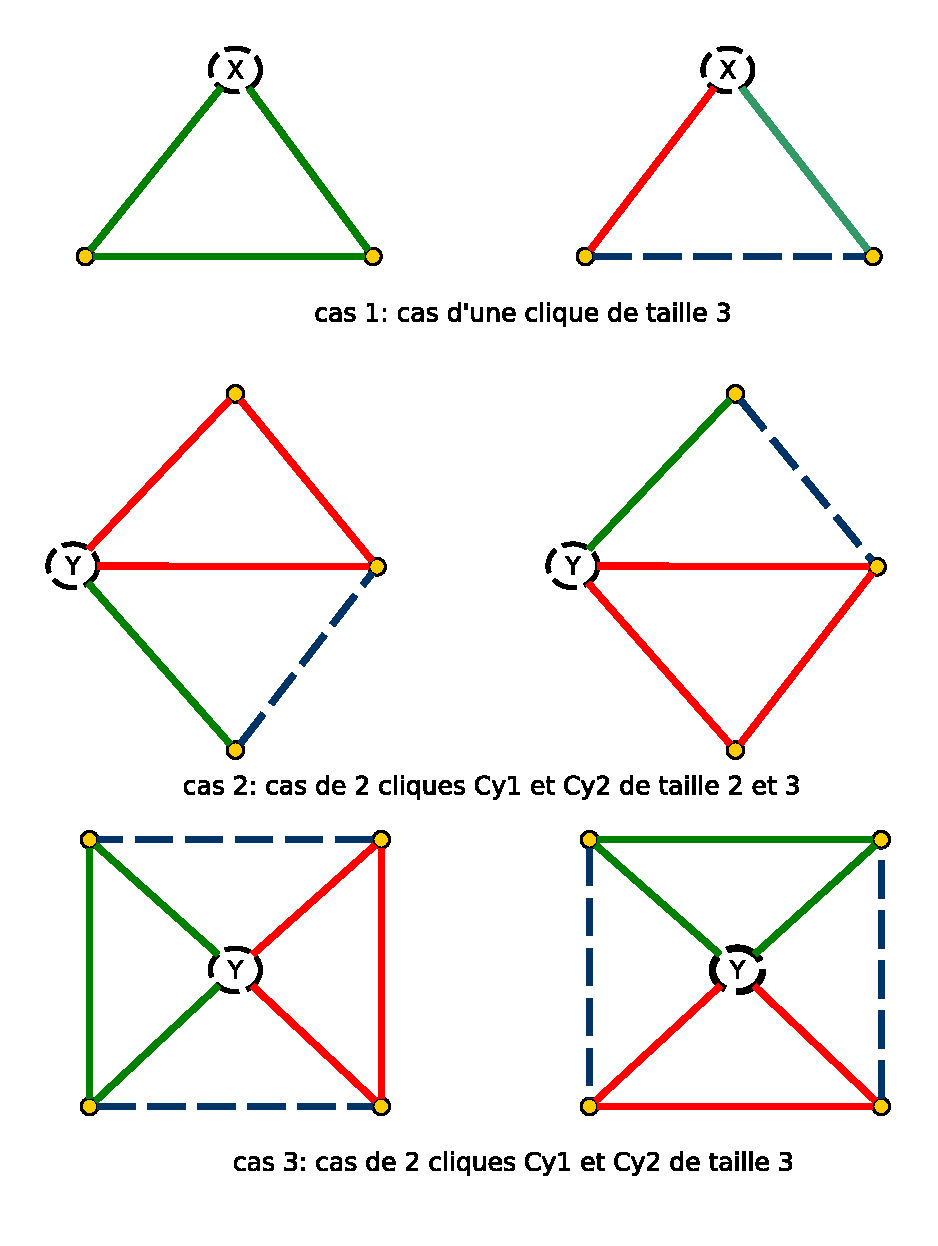
\includegraphics[scale=0.70]{configurationAmbiguite.eps}\vspace{-0.5em}
	\caption{ Configurations possibles d'une ambigu\"{i}t\'e au sommet X. }\vspace{-0.5em}
	\label{configurationAmbiguite}
\end{figure}
% ----- figure configurationAmbiguite
\FloatBarrier


En effet, si $G[\{u\} \cup \Gamma_{G}(u)]$ a une ambigu\"{i}t\'e, chaque ar\^ete, qui n'est pas li\'ee au point d'ambigu\"{i}t\'e, doit \^etre une ar\^ete d'une et une seule autre ambigu\"{i}t\'e de $G$. Et chaque sommet d'une ambigu\"{i}t\'e, qui n'est pas un point d'ambigu\"{i}t\'e, doit appartenir \`a une et une seule autre ambigu\"{i}t\'e de $G$ dont il n'est pas non  plus le point d'ambigu\"{i}t\'e.
De plus, chaque ar\^ete, n'\'etant pas couverte par les deux configurations de cliques possibles dans une ambigu\"{i}t\'e (les ar\^etes en pointill\'ees dans la figure \ref{configurationAmbiguite}), doit \^etre dans une autre ambigu\"{i}t\'e \`a laquelle elle appartient.
Ces contraintes font que si un graphe contient une ambigu\"{i}t\'e induite, alors il ne peut \^etre que dans un cas de la figure  \ref{graphe2Couverture}.

\begin{definition}
\label{cliquesCoherentes}
Soient $G$ un graphe, $u$ un sommet de $G$ et $\Gamma_G(u)$ les sommets voisins de $u$. 
\newline
Une partition de $\Gamma_G(u)$ en deux cliques $C_{u1}, C_{u2}$ est {\bf coh\'erente } si et seulement si chaque sommet $v$ de $C_{u1}$ (resp. $C_{u2}$) a au plus un voisin dans $C_{u2}$  (resp. $C_{u1}$).
\end{definition}

% ---- figure graphe de couverture
\begin{figure}[htb!] \vspace{-1.5em}
\centering
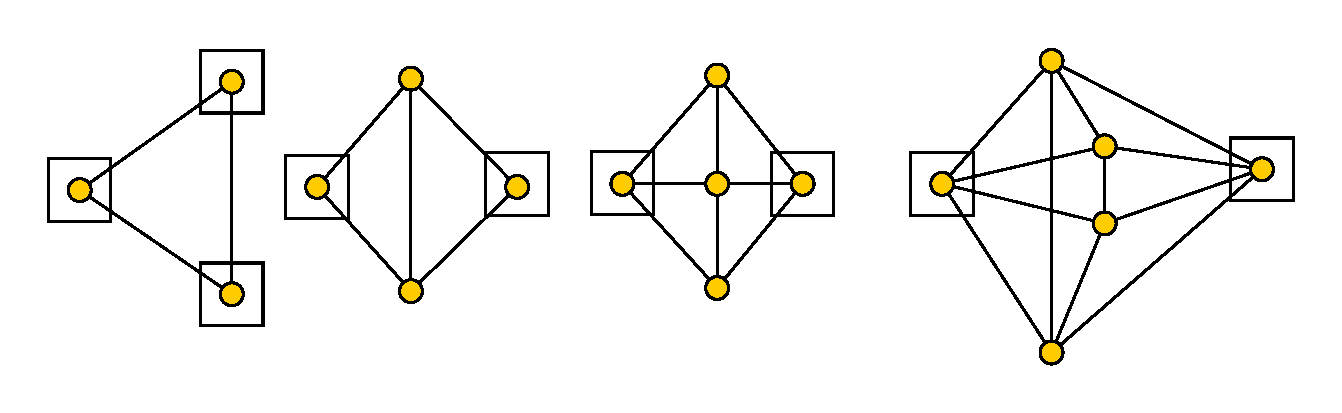
\includegraphics[scale=0.75]{graphe2Couverture.eps}
\caption{ Les graphes possibles de deux couvertures de corr\'elation avec les points d'ambigu\"{i}t\'es encadr\'es. }
\label{graphe2Couverture} 
\end{figure}
% ---- figure graphe de couverture
\FloatBarrier


{\bf Conclusion} : 
nous avons montr\'e que la {\em couverture de corr\'elation} d'un line-graphe est unique \`a l'exception des situations ambigu\"{i}t\'es. Les cas d'ambigu\"{i}t\'es sont pr\'esent\'es dans la figure \ref{graphe2Couverture}.


